\chapter{Background}
% Add maximum likelihood background explanation
% Add Bayesian probability background explanation
%Add note to say that we use the word examinee to mean someone taking a test although the test may not be an exam per say.

\section{Computer Based Tests}
CBT abbreviation
- offers advantages such as being able to display higher quality visuals such as pictures, videos, graphs, etc...
- low paperwork, everything is stored on the computer
- automatic grading, less work for teachers
- generation of statistics is made easier by the fact that the data can be processed by the computer
- nowadays a lot of learning is done on computer systems, and children are used to dealing with computers so assessment through this medium is advantageous. \newline

CBTs are typically "fixed-item" tests where all the students answer the same set of questions,  usually provided by the person responsible for the assessment. This isn't ideal since students can be presented with questions that are too easy or too difficult for them to answer. Consequently, the results of the test won't give a very accurate representation of a student's ability, and for this reason, these types of tests aren't extremely useful. This problem lead to research and the development of computerized adaptive testing (CAT).

\section{Computerized Adaptive Testing}
\label{sec:CAT}
Computerized adaptive testing (CAT), also called \textit{tailored testing}, is a form of computer-based testing which administers questions (referred to as \textit{items} in the psychometrics literature) of the appropriate difficulty by adapting to the examinee's ability.
For example, if an examinee answers an item correctly, then the next item presented will higher on the difficulty scale. On the other hand, if they answer incorrectly, they will be presented with an item lower on the difficulty scale. \newline

From an architectural perspective, a computerized adaptive test (CAT) consists of five components \cite{CAT-Framework}:

\subsubsection{1. Calibrated item pool}
An item pool is needed to store all the items available for inclusion in a test. This item pool must be calibrated with a psychometric model. During this phase, the item parameters are estimated according to the chosen model and scaled to fit with already existing items. Usually, the psychometric model employed in these systems is called Item Response Theory (IRT) (section \ref{subsec:IRT}). Calibration is a complex process, and to be done accurately it requires a considerable amount of data. Typically, it is performed by psychometricians, aided by expensive and sophisticated calibration software.

\subsubsection{2. Starting point}
Initially, when zero items have been administered, no information is known about the examinees and so the CAT is unable to estimate their ability. As a result, the item selection algorithm will fail to choose the next item to be administered.
If there is previous information available, for example an examinee's ability estimate in a closely related subject, then this can be input into the system to form the starting point configuration. Often this data isn't available or too costly to collect, so the CAT's initial ability estimate for the examinee corresponds to the mean on the ability scale - hence the first item presented will be of average difficulty.

\subsubsection{3. Item selection algorithm}
The item selection algorithm chooses the next item to present to the examinee based on the ability estimate of the examinee up to that point. Several methods exist and largely depend on the psychometric model in use. One of the most commonly used methods is the \textit{maximum information method} (section \ref{subsec:IRT}), which selects the item which maximizes the information function with respect to the estimated ability at that point.

\subsubsection{4. Scoring algorithm}
The scoring algorithm refers to the steps taken to update the examinee's ability estimate after an item has been answered. The two most commonly used methods are \textit{maximum likelihood estimation} (section \ref{subsec:IRT}) and \textit{Bayesian estimation} (section \ref{subsec:IRT}).

\subsubsection{5. Termination criterion}
The termination criterion specifies when the CAT should finish. For example the CAT can terminate when the change in the ability estimate after each iteration is below a certain threshold, or when time has run out, or when $N$ items have been administered, etc... Obviously, the CAT shouldn't be terminated too early, so as to allow enough time to estimate the examinee's ability with acceptable accuracy.

\begin{figure}[H]
\centering
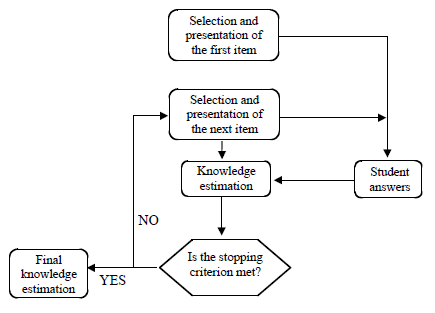
\includegraphics[scale=1]{cat_flowchart}
\caption{Flowchart of an adaptive test. Adapted from \cite{SIETTE}.}
\label{fig:cat_flowchart}
\end{figure}

The flowchart in figure~\ref{fig:cat_flowchart} corresponds to components 2-5, and illustrates the basics of the algorithm implemented in CAT. \cite{CAT-Wiki} gives a more detailed description of the procedure:
\begin{itemize}
\item[1.] The pool of items that haven't been administered yet is searched to determine the best item to present to the examinee, according to the current estimation of his ability.
\item[2.] The chosen item is presented to the examinee, who then answers it correctly or incorrectly.
\item[3.] The ability estimate is updated, based upon this new piece of information and the previous ability estimate.
\item[4.] Steps 1–3 are repeated until a termination criterion is met.
\item[5.] The algorithm returns a final ability estimate for the examinee's performance along with a confidence level: a percentage value indicating how accurate the estimate is.
\end{itemize}

CATs offer several advantages over traditional CBTs. As a result CATs have been used in many areas\cite{CAT-Areas}, such as education, job hiring, counselling, clinical studies, etc... Since CATs administer items by adapting to the examinee's ability, the test-taking experience ends up being a more positive one. Indeed, examinees won't have to deal with answering items which are too difficult or too easy compared to their ability level, a problem which appears in traditional CBTs.\newline

In addition, by administering only those items which will yield additional information, CATs end up being more accurate in estimating an examinee's ability level. This contrasts with CBTs which usually provide the best precision for examinees of medium ability, whereas extreme scores end up being less accurate.\newline

Lastly, CATs can come up with an ability estimate much quicker and with fewer administered items when compared to traditional CBTs. Indeed, an adaptive test can typically be shortened by 50\% and still maintain a higher level of precision than a fixed version.\cite{Weiss1984}
\newline

Despite the advantages mentioned above, CATs have some limitations. A frequent complaint is that an examinee isn't allowed to go back and change his answer to a past item. This limitation exists to prevent the examinee from intentionally answering items incorrectly to make subsequent items easier, and then going back and selecting the correct answers to achieve a perfect score. For similar reasons, it isn't possible to skip items, the examinee must select an answer to move on to the next item.\newline

The second issue has to do with the items themselves. First of all, there is the need for a large bank of items to cater to all ability levels. Developing an item pool of sufficient size can be very time consuming. David J. Weiss writes in \cite{Weiss1985} that item pools with 150-200 items are to be preferred, although 100 high quality items can sometimes be enough to achieve adequate estimations of ability levels.

Secondly, for the CAT to be of good quality the item pool needs to be calibrated accurately. This requires pre-administering the items to a sizeable sample and then simultaneously estimating all the item parameters for each item. The guidelines in \cite{CAT-Primer} suggest that sample sizes may be as large as $1000$ examinees. This phase is costly, time consuming and often times simply unfeasible.\newline

Lastly, item exposure is a possible security concern. Sometimes particular items may be presented too often and become overused. This may result in examinees becoming familiar with them and sharing them to other examinees of the same ability level, thus corrupting the results of the test. This problem can be solved to some extent by modifying the item selection algorithm to include some exposure control mechanism.\newline

A brief overview of CATs was given in this section. All of these concepts will be explored in more detail in item response theory (section \ref{subsec:IRT}) and in the implementation of adaptive testing in jSCAPE (chapter XX?).

\section{Probabilistic Test Theory}
In this section we go over a few topics in probability and how they can be implemented successfully in the area of computer assessments.

\subsection{Likelihood and Maximum Likelihood Estimation}
Although the terms probability and likelihood are used interchangeably in every day life, in statistics a distinction can be made.\newline

For any stochastic process, let us denote the observed outcomes as $x$ and the set of parameters as $\theta$. When we say probability, we want to calculate $P(x | \theta)$, i.e. the probability of observing the outcomes $x$ given specific values for the set of parameters $\theta$. \newline



In more mathematical terms, we have:
$$L(\theta | x) = P(x | \theta)$$

To highlight the distinction we illustrate with an example of how the two terms are used. If we consider a dice, a possible parameter is the fairness of the dice, while possible outcomes are which values are displayed after a roll. For instance, if a fair dice is rolled 5 times, what is the \textit{probability} that a 6 will show up on every roll? If a dice is rolled 5 times and lands on 6 every roll, what is the \textit{likelihood} that the dice is fair? \newline

Maximum likelihood estimation refers to a method of statistical inference where one can find the set of parameter values ($\theta$) which are most \textit{likely} given the observed outcomes ($x$). As mentioned in the name of the method, this is done by finding the parameter values which maximize the likelihood function $L(\theta | x)$.

\subsection{Bayes probability theory}
% Add maximum likelihood background explanation
% Conditional probability quick overview?
% Add Bayesian probability background explanation
% Bayesian networks
% Latent variables ?

\subsection{Item Response Theory}
\label{subsec:IRT}
We mentioned in section \ref{sec:CAT} that Item Response Theory (IRT) is usually the psychometric model of choice when developing a CAT, e.g. the Graduate Record Examination (GRE) and Graduate Management Admission Test (GMAT). CATs can still be implemented with Classical Test Theory but they offer less sophistication and less information to evaluate/improve the reliability of the test, making IRT the superior choice. \newline

IRT attempts to model the answer to an item as a mathematical model. \newline

Several IRT models have been developed over the years to address the different types of tests that exist, e.g. multiple choice exams, agreement questionnaires (Likert scale), etc... These models all seek to achieve the same goal, modelling the examinee's ability on some ability scale, but they differ in the number of parameters associated with each item. We now take a greater look at these different models:

\subsubsection{The one-parameter logistic model}
\begin{equation} \label{eq:1PL-IRF}
P(\theta) = \frac{1}{1 + \me^{-(\theta - b)}}
\end{equation}

Equation \eqref{eq:1PL-IRF} shows the item response function for the one-parameter logistic model (1PL). 

\subsubsection{The two-parameter logistic model}
\begin{equation} \label{eq:2PL-IRF}
P(\theta) = \frac{1}{1 + \me^{-1.7a(\theta - b)}}
\end{equation}

Equation \eqref{eq:2PL-IRF} shows the item response function for the two-parameter logistic model (2PL). 

\subsubsection{The three-parameter logistic model}
\begin{equation} \label{eq:3PL-IRF}
P(\theta) = c + \frac{1 - c}{1 + \me^{-1.7a(\theta - b)}}
\end{equation}

Equation \eqref{eq:3PL-IRF} shows the item response function for the three-parameter logistic model (3PL). 

\subsubsection{Estimating the ability}
In section \ref{sec:CAT}, when discussing scoring algorithms, we saw that the two most common methods for ability estimation were \textit{maximum likelihood estimation} and \textit{Bayesian estimation}.\newline

In the \textit{maximum likelihood estimation} method, we need to define a likelihood function in terms of the ability level ($\theta$) we are trying to estimate:

\begin{equation} \label{eq:Trait-estimation}
L(\theta | \textbf{u}) = L(\theta | u_1, ..., u_n) = P(u_1, ..., u_n | \theta) = \prod_{i=1}^n P_i(\theta)^{u_i}(1 - P_i(\theta))^{(1 - u_i)} ,
\end{equation}

where $\textbf{u}=(u_1, ..., u_n)$ is called the reponse vector for an examinee, that is $u_i=1$ if the examinee answers the i$^\text{th}$ item correctly, and $u_i=0$ if the examinee answers the i$^\text{th}$ item incorrectly. $P_i(\theta)$ corresponds to the probability of answering the i$^\text{th}$ item correctly when the ability level is $\theta$, and thus $1 - P_i(\theta)$ gives the probability of answering the i$^\text{th}$ item incorrectly when the ability level is $\theta$. \newline

Now that the likelihood function is defined, we can apply maximum likelihood estimation to find the ability level which is most likely given the examinee's response vector. Let us illustrate with a very simplistic example where ability levels are discrete values between $-1$ and $+1$. We would iterate through these ability levels and compute the following values, for example:
\begin{align*}
L(\theta=-1 | \textbf{u}) &= 0.001 \\
L(\theta=+0 | \textbf{u}) &= 0.012 \\
L(\theta=+1 | \textbf{u}) &= 0.054
\end{align*}

The likelihood function is maximized when $\theta = +1$, and so this is the maximum likelihood estimate for $\theta$. In a CAT, and based on the examinee's response vector \textbf{u}, the system would assign $+1$ as the ability level for that examinee.\newline

The \textit{Bayesian estimation} method is also somewhat based on the likelihood function and therefore very similar to \textit{maximum likelihood estimation}.........


\subsubsection{Item information}

\section{Summary}
We have gone over types of computer based assessment and how they differ from regular assessment techniques. We have also provided an overview of the theoretical components and probability concepts which will be implemented in jSCAPE (chapter xx?).
